\documentclass{beamer}
%\documentclass[handout]{beamer}
% This file is a solution template for:

% - Giving a talk on some subject.
% - The talk is between 15min and 45min long.
% - Style is ornate.
% Copyright 2004 by Till Tantau <tantau@users.sourceforge.net>.
%
% In principle, this file can be redistributed and/or modified under
% the terms of the GNU Public License, version 2.
%
% However, this file is supposed to be a template to be modified
% for your own needs. For this reason, if you use this file as a
% template and not specifically distribute it as part of a another
% package/program, I grant the extra permission to freely copy and
% modify this file as you see fit and even to delete this copyright
% notice. 

\mode<presentation>
{
  \usetheme{Montpellier}

  %\setbeamercovered{transparent}
  % or whatever (possibly just delete it)
}

\usepackage{xmpmulti} % package that defines \multiinclude
\usepackage{amsmath,amsfonts,amsthm,bm}

\usepackage[english]{babel}

\usepackage[latin1]{inputenc}

\usepackage{times}
\usepackage[T1]{fontenc}
% Or whatever. Note that the encoding and the font should match. If T1
% does not look nice, try deleting the line with the fontenc.

\title[\ouralg] % (optional, use only with long paper titles)
{Mirror Descent}

\author[Freund] % (optional, use only with lots of authors)
{Yoav Freund}
% - Give the names in the same order as the appear in the paper.
% - Use the \inst{?} command only if the authors have different
%   affiliation.

\institute[Universities of Somewhere and Elsewhere] % (optional, but mostly needed)

\subject{Machine Learning}

\beamerdefaultoverlayspecification{<+->}

\newcommand{\newmcommand}[2]{\newcommand{#1}{{\ifmmode {#2}\else\mbox{${#2}$}\fi}}}
\newcommand{\newmcommandi}[2]{\newcommand{#1}[1]{{\ifmmode {#2}\else\mbox{${#2}$}\fi}}}
\newcommand{\newmcommandii}[2]{\newcommand{#1}[2]{{\ifmmode {#2}\else\mbox{${#2}$}\fi}}}
\newcommand{\newmcommandiii}[2]{\newcommand{#1}[3]{{\ifmmode {#2}\else\mbox{${#2}$}\fi}}}

\newcommand{\algfnt}{\bf}

\newmcommand{\ouralg}{{\mbox{\algfnt Hedge}({\eta})}}

\newmcommand{\iter}{T}

\newfont{\cmmib}{cmmib10}
\newcommand{\boldell}{{\mbox{\cmmib \symbol{'140}}}}

\newmcommandi{\costvec}{{\boldell}^{#1}}
\newmcommandii{\cost}{{\ell}^{#1}_{#2}}

\newmcommandi{\rd}{\tilde{#1}}

\newmcommandi{\distvec}{{\bf p}^{#1}}
\newmcommandi{\rddistvec}{\rd{\bf p}^{#1}}
\newmcommandii{\dist}{{p}^{#1}_{#2}}
\newmcommandii{\rddist}{\rd{p}^{#1}_{#2}}

\newmcommandi{\bdistvec}{{\bf q}^{#1}}
\newmcommandii{\bdist}{{q}^{#1}_{#2}}

\newmcommandi{\wtvec}{{\bf w}^{#1}}
\newmcommandi{\rdwtvec}{\rd{\bf w}^{#1}}
\newmcommandii{\wt}{{w}^{#1}_{#2}}
\newmcommandii{\rdwt}{\rd{w}^{#1}_{#2}}

\newcommand{\w}[1]{\makebox[12pt]{{#1}}}
\newcommand{\Rps}{\mbox{\tt R}}
\newcommand{\rPs}{\mbox{\tt P}}
\newcommand{\rpS}{\mbox{\tt S}}
\newcommand{\rpstie}{\w{$\frac{1}{2}$}}
\newcommand{\rpswin}{\w{$0$}}
\newcommand{\rpsloss}{\w{$1$}}

\newmcommand{\decspace}{\Delta}
\newmcommand{\decsym}{\delta}
\newmcommandi{\dec}{\decsym^{#1}}
\newmcommand{\decdistsym}{\cal D}
\newmcommandi{\decdist}{{\decdistsym}^{#1}}

\newmcommand{\simpdistspace}{{\bf \cal S}}
\newmcommand{\domset}{{\rm dom}(\decdistsym)}

\newmcommand{\expdistsym}{{\cal E}}
\newmcommandii{\expdist}{{\expdistsym}^{#1}_{#2}}
\newmcommand{\expdecsym}{{\varepsilon}}
\newmcommandii{\expdec}{\expdecsym^{#1}_{#2}}

\newmcommand{\outspace}{\Omega}
\newmcommand{\outsym}{\omega}
\newmcommandi{\out}{\outsym^{#1}}

%\newmcommandii{\Dkl}{D_{\mbox{kl}}\paren{#1||#2}}
\newmcommandii{\Dkl}{{\rm {KL}}\paren{{#1}\;||\;{#2}}}

\newmcommandi{\sumwts}{\sum_{i=1}^N \wt{#1}{i}}

\newmcommand{\lossalg}{L_A}
\newmcommand{\lossouralg}{{L_{\mbox{\scriptsize\algfnt Hedge}(\eta)}}}
\newmcommand{\lossS}{{L_{\mbox{\scriptsize\algfnt S}}}}
\newmcommandi{\lossi}{L_{#1}}
\newmcommandii{\lossit}{L_{#1}^{#2}}

\newmcommandi{\upbnd}{\tilde{#1}}

\newcommand{\angles}[1]{{\left\langle {#1} \right\rangle}}
\newcommand{\paren}[1]{{\left( {#1} \right)}}
\newcommand{\abs}[1]{{\left| {#1} \right|}}
\newcommand{\ceiling}[1]{{\left\lceil {#1} \right\rceil}}

\newfont{\msym}{msbm10}
\newcommand{\real}{\mbox{\msym R}}

\newmcommand{\updatefcn}{U_\eta}

%% \newtheorem{theorem}{Theorem}	
%% \newtheorem{lemma}[theorem]{Lemma}
%% \newtheorem{corollary}[theorem]{Corollary}
%% \newtheorem{definition}{Definition}

%\newcommand{\proof}{\noindent{\bf Proof:} }
%\newcommand{\example}[1]{{\em Example #1.} }
%\newcommand{\qed}{\rule{0.7em}{0.7em}}

\newcommand{\WeakAlg}{\mbox{\algfnt WeakLearn}}
\newcommand{\Boost}{\mbox{\algfnt AdaBoost}}
\newcommand{\EX}{\mbox{\bf EX}}
\newmcommand{\hf}{h_{{f}}}
\newmcommand{\rdhf}{\rd{h}_{{f}}}
\newmcommand{\hfT}{h^T_{{f}}}
\newmcommand{\ranh}{{b}}

\newmcommand{\conclass}{{\cal C}}

\newmcommand{\badvec}{{\bf b}}
\newmcommandi{\bad}{{b}_{#1}}

%%%%%%%% New commands defined for the game-playing paper

\newmcommand{\hedge}{\algfnt Hedge}
\newmcommand{\play}{\algfnt Play}
\newmcommandi{\Glossvec}{{\bg y}^{#1}}
\newmcommandii{\Gloss}{{y}^{#1}_{#2}}
%\newmcommandi{\action}{{I}_{#1}}
\newmcommandi{\Gdistvec}{{\bf \tilde{p}}^{#1}}
\newmcommandii{\Gdist}{{\teilde{p}}^{#1}_{#2}}

%%%%%%%%%%%%%%%%%%%%%%%%%%%%%%%%%%%%%%%%%%%%%%%%%%%%%
\newmcommand{\Idistvec}{{D}}
\newmcommandi{\Idist}{\Idistvec({#1})}
\newmcommand{\Idistt}{\Idistvec_t}

\newmcommand{\Xdist}{{\cal P}}
\newmcommand{\emp}{\hat{\epsilon}}

\newmcommand{\classpc}{Y}
\newmcommand{\numclass}{k}
\newmcommandii{\prob}{\mbox{\rm Pr}_{#1}\left[{#2}\right]}
\newmcommandii{\exval}{\mbox{\rm E}_{#1}\left[{#2}\right]}

\newmcommand{\lab}{y}
\newmcommand{\ploss}{\mbox{ploss}}
\newmcommandii{\avploss}{\ploss_{#1}({#2})}
\newcommand{\sfrac}[2]{\mbox{$\frac{#1}{#2}$}}

\newcommand{\mboosta}{\mbox{\algfnt AdaBoost.M1}}
\newcommand{\mboostb}{\mbox{\algfnt AdaBoost.M2}}
\newcommand{\mboostr}{\mbox{\algfnt AdaBoost.R}}

\newmcommand{\slos}{\mbox{ploss}}
\newmcommandiii{\sloss}{\slos_{#1}({#2},{#3})}
\newmcommandiii{\avsloss}{\slos_{{#1},{#2}}({#3})}

\newmcommandii{\vwt}{{W}^{#1}_{#2}}

\newcommand{\figline}{\rule{\textwidth}{1pt}}

%\newmcommandi{\1}{{\bf 1}({#1})}
\newmcommandi{\1}{[\![{#1}]\!]}

\newmcommand{\confcn}{\kappa}
\newmcommandi{\erint}{\abs{\int_{y_i}^{h_t(x_i)} {#1} dy}}
%\newmcommandi{\erint}{\int_{\min\{y_i,h_t(x_i)\}}^{\max\{y_i,h_t(x_i)\}}{#1}dy}


\begin{document}

%\iffalse %%%%%%%%%%%%%%%%%%%%%%%%%%%%%%%%%%%%%%%%%%%%%%%%%%%%%%%%%%%%%%%%%%
%\fi %%%%%%%%%%%%%%%%%%%%%%%%%%%%%%%%%%%%%%%%%%%%%%%%%%%%%%%%%%%%%%%%%%%

\begin{frame}
  \titlepage
  \begin{small}
    Material follows Chapter 11 of ``Prediction Learning and
    Games'' Sections 11.\{1,2,3\}
  \end{small}
\end{frame}

\begin{frame}
  \frametitle{Outline}
  \tableofcontents[pausesections]
  % You might wish to add the option [pausesections]
\end{frame}

\section{Linear Pattern Recognition}
\begin{frame}
  \frametitle{Linear Pattern Recognition}
  \begin{itemize}
  \item Instance: \R{$(\vx_t,y_t) \in \real^d \times \real$}
  \item Expert: \R{$\vu \in \real^d$}
  \item Predictor: \R{$\vw_t \in \real^d$}
  \item Loss \R{$\ell(\vw\cdot \vx,y)$} (online regression = square loss)
  \item Regret: \R{$\RR_t(\vu) = 
      \sum_{i=1}^t  \left[ \ell(\vw_t\cdot \vx_t,y_t)
        - \ell(\vu \cdot \vx_t,y_t)\right]$}
  \end{itemize}
\end{frame}

\section{Potential Based Gradient descent}


\begin{frame}
  \frametitle{Potential based gradient Descent}
  \begin{itemize}
  \item \R{$\RR_t$} = Regret vector \R{$R_t(\vw) = L_{A,t} - L_t (\vw)$}
  \item \R{$\RR_t$} = State of prediction algorithm at time \R{$t$}
  \item Potential: \R{$\Phi(\RR)$} Quantifies \B{badness} of the
    state.
  \item A state is bad if adversary can force high regret in the future.
  \item Choose prediction to balance \R{$\Phi(\RR_{t+1}) - \Phi(\RR_t)
      + \vw_t \cdot \lossvec{t}$} is small for all possible \R{$\lossvec{t}$}
  \item \R{$\vw_t = \nabla \Phi(\RR_t)$} is a good choice.
  \item For finite number of experts, \R{$\RR_t$} is finite
    dimensional and we can compute \R{$\vw_t$} explicitly.
  \item Here, \R{$\RR = \{R(\vw)\}_{\vw \in \real^d}$} is continuous
    dimensional.
  \item Experts that correspond to exponential distributions - we can
    use conjugate priors. (recall: biased coins).
  \item We need a new trick to compute \R{$\vw_t = \nabla \Phi(\RR_t)$} efficiently.
  \end{itemize}
\end{frame}

\section{Duality}

\begin{frame}
\frametitle{Dual Vector Spaces}

\begin{itemize}
\item \R{$V$} is a vector space, with a norm \R{$\|v\|$}
\item \R{$U$} is the set of all linear mappings from \R{$V$} to
  \R{$V$}
  \item
  The norm of \R{$u \in U$} is defined as
  \R{$$\|u\|^* = \max_{v \in V} \frac{\|u(v)\|}{\|v\|}$$}
\item \R{$V$} is equivalent to the set of all linear mappings from \R{$U$} to
  \R{$U$}.
\item \R{$U$} and \R{$V$} are dual vector spaces, with dual norms. 
\end{itemize}
\end{frame}

\begin{frame}
\frametitle{Dual Norms}
\begin{itemize}
  \item The space is always \R{$U,V = \real^n$}
  \item The linear operation is the dot product \R{$\vu \cdot \vv$}
\item \R{$L_2$} norm: \R{$\sqrt{\sum_{i=1}^n x_i^2}$}
\item \R{$L_1$} norm: \R{$\sum_{i=1}^n |x_i|$}
\item \R{$L_\infty$} norm: \R{$\max_i |x_i|$}
\item \R{$L_p$} norm: \R{$\paren{\sum_{i=1}^n x_i^p}^{\frac{1}{p}}$}
\item \R{$L_p,L_q$} are dual norms if \R{$p,q \geq 1, \mbox{ and }\frac{1}{p} + \frac{1}{q} = 1$}
\item \R{$L_1,L_\infty$} are dual.
\item \R{$L_2$} is self-dual. 
\end{itemize}
\end{frame}

\begin{frame}
\frametitle{Fenchel Duality}
\begin{itemize}
  \item \R{Fenchel duality allows non-differentiable functions and uses sub-gradient}
\item Suppose \R{$F:A \to \real$} is a convex function over a convex set \R{$A
    \subseteq \real^n$}.
\item The dual function to \R{$F$} is
  \R{$$
    F^*(\vu) = \sup_{\vv \in A}\paren{\vu \cdot \vv -F(\vv)}
$$}
\end{itemize}
\end{frame}

\begin{frame}
  \frametitle{Visualization for \R{$\real$}}
  \begin{columns}
    \begin{column}{0.55\textwidth}
        \begin{itemize}
            \item \R{$x,y \real$}
            \item \R{$ f^*(y) = \sup_{x \in \real}\paren{xy-f(x)}$}
            \item \R{$ -f^*(y) = \inf_{x \in \real}\paren{f(x)-xy}$}
        \end{itemize}
    \end{column}
    \begin{column}{0.43\textwidth}
          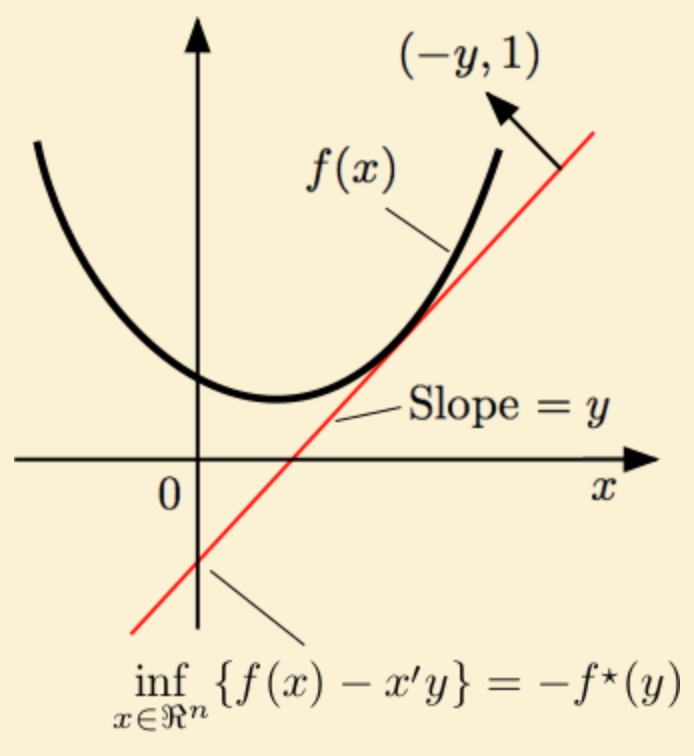
\includegraphics[width=\textwidth]{figures/Legendre-Duality.png}
    \end{column}
\end{columns}
\end{frame}

\begin{frame}
  \frametitle{Dual of Dual}
  \begin{itemize}
  \item The dual of any function is convex.
  \item if \R{$F$} is convex then \R{$F^{**} = F$}
  \end{itemize}
  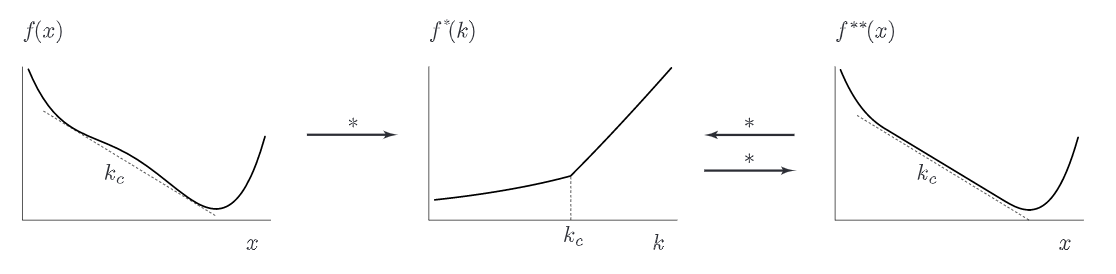
\includegraphics[width=\textwidth]{figures/FromNonConvexToConvex.png}  
\end{frame}

\begin{frame}
  \frametitle{Gradient Duality}
  \begin{itemize}
  \item
    If the gradient of \R{$f$} at \R{$x$} is \R{$k$} then\\
    the gradient of \R{$f^*$} at \R{$k$} is \R{$x$}
    \item In general:
  \R{$$
    \nabla F^* = \paren{\nabla F}^{-1}
    $$}
  \end{itemize}
  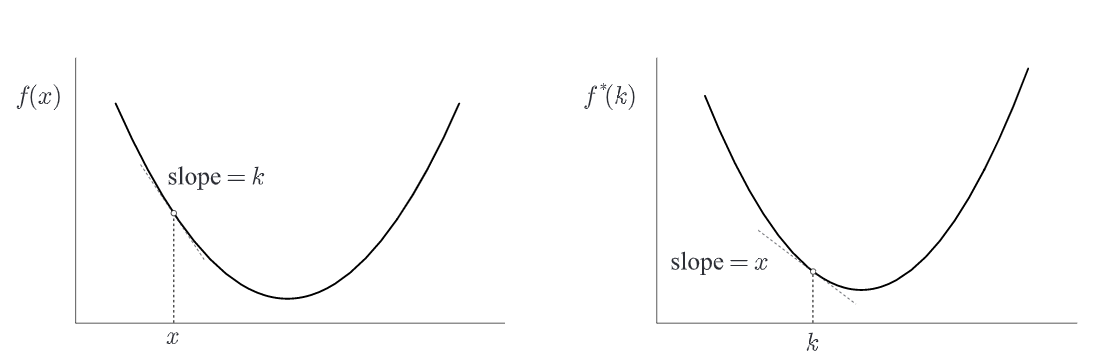
\includegraphics[width=\textwidth]{figures/SlopeDuality.png}
\end{frame}

\begin{frame}
  \frametitle{Example: Exponential Potential}
  \begin{itemize}
  \item Potential: \R{$F(\vu) = \sum_{i=1}^d e^{u_i}$}
  \item Gradient: \R{$\nabla F(\vu)_i = e^{u_i}$} or \R{$\nabla F(\vu)
      = F(\vu)$}.
  \item Dual:  \R{$F^*(\vv) = \sum_{i=1}^d v_i (\ln v_i -1)$}
  \item Gradient of dual: \R{$\nabla F^*(\vv)_i = \ln v_i $} 
  \item Note \R{$(\nabla F)^{-1} = \nabla F^*$}
   \end{itemize}
 \end{frame}

\begin{frame}
  \frametitle{Fenchel and Bregman}
  \begin{itemize}
  \item
    \R{$F$}: strictly convex with continuous first derivative.
  \item \R{$F^*$} is the Fenchel Dual of \R{$F$}
  \item \R{$D_F,D_{F^*}$} Bregman divergences wrt \R{$F,F^*$}
  \item \R{$\vu' = \nabla F(\vu)$} and \R{$\vv' = \nabla F(\vv)$}
  \item \R{$D_F(\vu,\vv)  = D_{F^*}(\vu',\vv')$}
  \end{itemize}
\end{frame}

\section{The Mirror Descent Algorithm}

\begin{frame}
  \frametitle{Dual parameters}
  \begin{itemize}
  \item We want to compute
    \R{$\vw_t = \nabla \Phi(\RR_t)$}
  \item Let \R{$\Phi^*$} by the convex Dual of \R{$\Phi$}
  \item \R{$\RR_t = \nabla \Phi^*(\vw_t)$}
    \item We use \R{$\Btheta_t =\RR_t$} because we treat \R{$\RR_t$} as a parameter.
  \item \R{$\rr_t$} regret for single step.
  \item \R{$\Btheta_t = \Btheta_{t-1} + \rr_t$}
  \item re-written using Duality:
    \R{$$
    \nabla \Phi^*(\vw_t) = \nabla \Phi(\vw_{t-1}) + \rr_t
    $$}
  \end{itemize}
\end{frame}

\begin{frame}
  \frametitle{Mirror Descent}
  \begin{itemize}
  \item Gradient descent in dual space
    \R{$\Btheta_t = \Btheta_{t-1} - \lambda \nabla \ell_t(\Btheta_{t-1})$}
  \item Using duality can be rewritten as
    \R{$$\nabla \Phi^*(\vw_t) =  \nabla \Phi^*(\vw_{t-1})  - \lambda \nabla \ell_t(\vw_{t-1})$$}
  \item As \R{$\nabla \Phi$} is the inverse of \R{$\nabla \Phi^*$} we get
    \R{$$ \vw_t = \nabla \Phi \paren{\nabla \Phi^*(\vw_{t-1})  - \lambda \nabla \ell_t(\vw_{t-1})}$$}
  \end{itemize}
\end{frame}

\begin{frame}
  \frametitle{A picture of mirror descent}
\R{$$ \vw_t = \nabla \Phi \paren{\nabla \Phi^*(\vw_{t-1})  - \lambda \nabla \ell_t(\vw_{t-1})}$$}
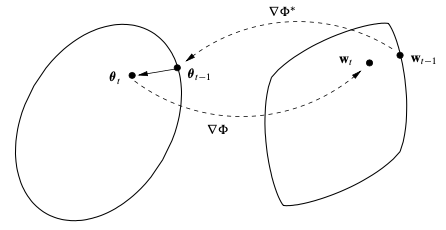
\includegraphics[width=\textwidth]{figures/MirrorDescent.png}
\end{frame}

\begin{frame}
  \frametitle{Intuition}
  \begin{itemize}
  \item \R{$\vu$} should balance minimizing the loss from observing same example again
    and divergence between \R{$\vu$} and \R{$\vw_{t-1}$}
  \item Exact Goal:
    \R{$\min_{\vu \in \real^d} \brac{D_{\phi^*} (\vu, \vw_{t-1})
        - \lambda \nabla \ell_t(\vu)}$}
  \item Taylor order one approximation:
    \R{$\min_{\vu \in \real^d} \brac{F(\vu)}$} where \\
    \R{$ F(\vu) = D_{\phi^*} (\vu, \vw_{t-1})
        - \lambda \brac{\ell_t(\vw_{t-1}) + (\vu-\vw_{t-1}) \nabla
          \ell_t(\vw_{t-1}) }$}
    \item Assuming everything is differrentiable and convex, \R{$
        \nabla_{\vu} F[\vu] = 0$} yields:
      \R{$\nabla \Phi^*(\vw_t) = \nabla \Phi^*(\vw_{t-1})  - \lambda \nabla \ell_t(\vw_{t-1}) $}
    \item Equivelently: \R{$\vw_t = \nabla \Phi \paren{\nabla \Phi^*(\vw_{t-1})  - \lambda \nabla \ell_t(\vw_{t-1})}$}
  \end{itemize}
\end{frame}

\begin{frame}
  \frametitle{Theorem}
  \begin{itemize}
  \item \R{$\ell:\real \times \real \to \real$} is a \B{regular}
    loss function if it is convex, non-negative and differentiable.
  \item Instantaneous Loss: \R{$\ell_t(\vw) = \ell(\vw \cdot \vx_t,y_t)$}
  \item Regret: \R{$\RR_t(\vu) = L_{A,t} - L_t(\vu)$}
  \item Theorem: For all example sequences
    \R{$(\vx_1,y_1),\ldots,(\vx_T,y_T)$}, any initial vector
    \R{$\vw_0 \in \real^d$}. all \R{$\lambda>0$} and all \R{$\vu \in \real^d$}:
    \R{$$
      \RR_T(\vu) \leq
      \frac{1}{\lambda} D_{\Phi^*}(\vu,\vw_0) +
      \frac{1}{\lambda} \sum_{t=1}^T D_{\Phi^*}(\vw_{t-1},\vw_t)
      $$}
  \end{itemize}
\end{frame}

\section{Algorithms for specific potentials}

\begin{frame}
  \frametitle{Polynomial Potential}
  \begin{itemize}
  \item Potential: \R{$\Phi_p(\vu) = \frac{1}{2} \|\vu\|_p^2= \frac{1}{2} \paren{\sum_{i=1}^d
        u_i^p}^{2/p}$}
  \item Dual Potential \R{$\Phi_p^* = \Phi_q$} Where
    \R{$\frac{1}{p}+\frac{1}{q} = 1$}
  \item Euclidean norm: \R{$q=p=2$}
  \item Suppose the sequence of examples
    \R{$(\vx_1,y_1),\ldots,(\vx_T,y_T)$} satisfies \R{$\| \vx_t \|_p
      \leq X_p$} for all \R{$1 \leq t \leq T$}
  \item Suppose we use the dual descend algorithm for the potential
    function \R{$\Phi_p$} and the learning rate \R{$\lambda =
      \frac{2 \epsilon}{(p-1) X_p^2}$} for some \R{$0<\epsilon<1$}
  \item \B{Loss Bound}:\\
    \R{$L_{A,T}  \leq \frac{L_T(\vu)}{1-\epsilon} + \frac{\| \vu
        \|_q^2}{\epsilon (1-\epsilon)}\times \frac{(p-1)X_p^2}{4}$}
  \end{itemize}
\end{frame}

\begin{frame}
\frametitle{Exponential Potential}
  \begin{itemize}
  \item Potential: \R{$\Phi(\vu) = \sum_{i=1}^d e^{u_i}$}
  \item Dual Potential \R{$\Phi^*(\vu) = \sum_{i=1}^d u_i (\ln u_i -1)$}
  \item Euclidean norm: \R{$q=p=2$}
  \item Suppose the sequence of examples
    \R{$(\vx_1,y_1),\ldots,(\vx_T,y_T)$} satisfies \R{$\| \vx_t \|_\infty
      \leq X_p$} for all \R{$1 \leq t \leq T$}
  \item Suppose we use the dual descend algorithm for the exponential potential
    function \R{$\Phi$} and the learning rate \R{$\lambda =
      \frac{2 \epsilon}{X_{\infty}^2}$}  for some \R{$0<\epsilon<1$}
  \item \B{Loss Bound}:\\
    \R{$L_{A,T}  \leq \frac{L_T(\vu)}{1-\epsilon} + \frac{X_\infty^2
        \ln d}{2 \epsilon (1-\epsilon)}$}
  \end{itemize}
\end{frame}

\end{document}


